\subsection{Compton}
High energy photons such as those from the transitions with \unit{122}{keV} and \unit{136}{keV} lose energy when passing through matter via the Compton effect. Some of these photons will randomly fall within the energy windows that was set for the measurements and thus pose an underground that needs to be subtracted from the data for parts of the further analysis. Since higher energy photons lose their energy slower than lower energy photons when passing through matter, one can separate the two by placing aluminum plates in the beam with a range of thicknesses. The count rate decreases exponentially with the thickness $d$ 
\begin{equation}
\dot{N}=\dot{N}_0e^{-\mu d}
\end{equation}
measurements were taken for absorber thicknesses between $d=\unit{0.21}{mm}$ and $d=\unit{12.43}{mm}$, which were measured with a caliper to such high precision that the error is far smaller than the Poisson error on the count rates and is thus neglected. Figure \ref{fig:comptonbackground} shows the measured data.
\begin{figure}
\centering
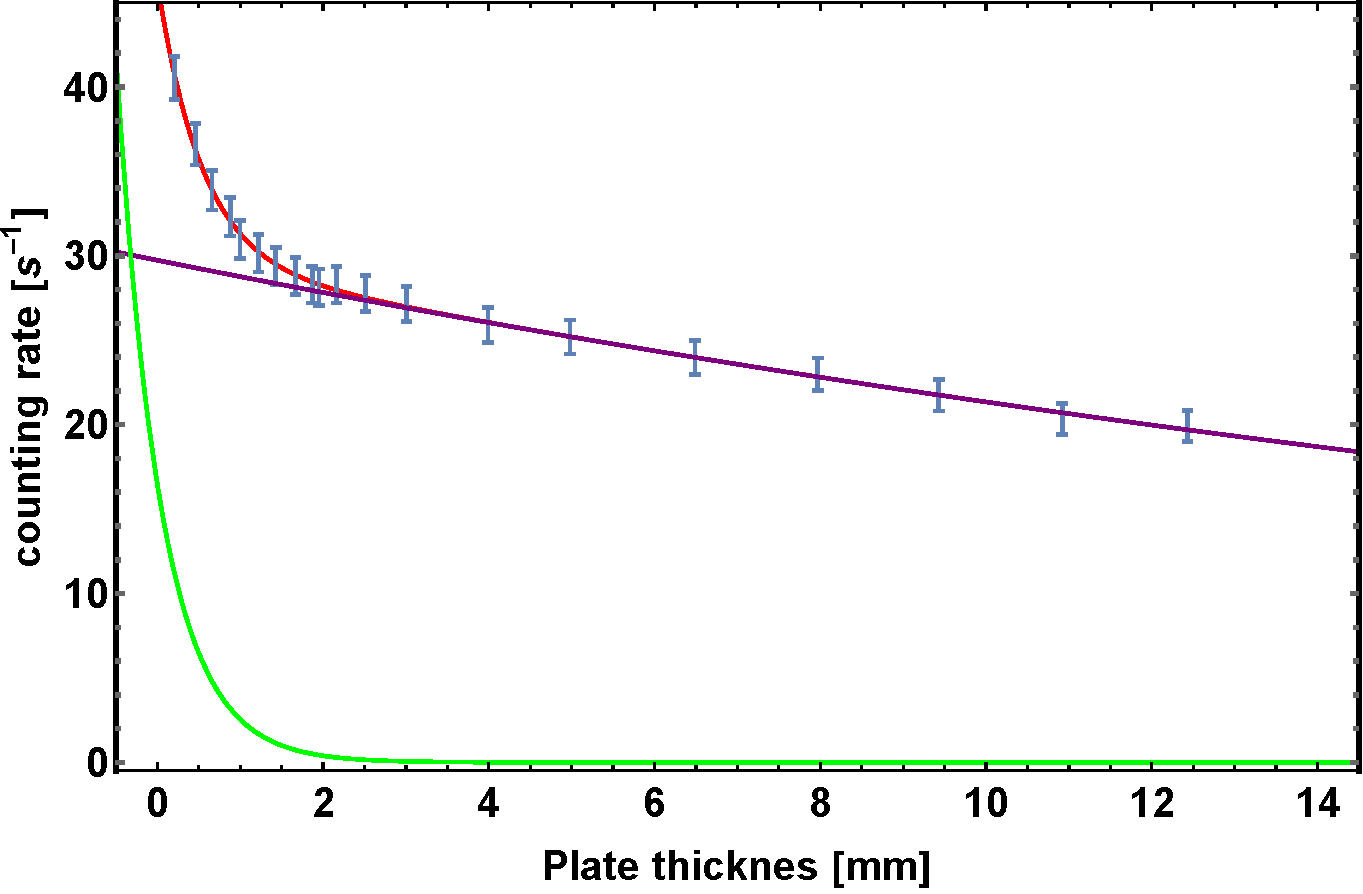
\includegraphics[width=1.0\linewidth]{graphics/comptonbackground}
\caption[Compton background data]{The compton background data along with the fitted sum of the two exponential functions in red. The curve for Compton underground is colored purple and that for the \unit{14,4}{keV} photons green.}
\label{fig:comptonbackground}
\end{figure}
As two processes with different speeds, $\mu_{C}$ of the Compton background and $\mu_0$ of the actual data, are expected, the fit function for the count rates for varying absorbers is
\begin{equation}
\dot{N}(d)=A_C\cdot e^{-\mu_C d}+A_0\cdot e^{-\mu_0 d}
\end{equation}
The resulting fit parameters for the Compton underground were
\begin{align}
A_C&=\unit{(29.74\pm0.17)}{s^{-1}}\\
\mu_C&=\unit{(0.0331\pm0.0009)}{mm^{-1}}
\end{align}
As no aluminum plates are used during regular measurements, the value for $d=0$, and thus the fit parameter $A_C$, is the underground rate to be deducted from future measurements.

\subsection{Attenuation of the acrylic glass}
The acrylic glass in which the sample is cased absorbs some of the radiation. To quantify this, a plate of acrylic glass of roughly the same thickness as the one used to case the sample can be but into the beam. One measurement is taken with the plate and one without. The thickness of the plate was measured as $d=\unit{(1.94\pm0.01)}{mm}$. The resulting count rates were
\begin{align}
\dot{N}_0&=\unit{(107.4\pm0.3)}{s^{-1}}\\
\dot{N}_A&=\unit{(84.8\pm0.3)}{s^{-1}}
\end{align}
where the uncertainties stem from the Poisson errors on the number of counts. The attenuation coefficient can then be calculated:
\begin{equation}
\mu_{acr}=Log\left[\frac{\dot{N}_0}{\dot{N}_A}\right]\cdot\frac{1}{d}=\unit{(1.21\pm0.02)}{1/cm}
\end{equation}
With the values given for the attenuation coefficient $\mu/\rho=\unit{1.101}{cm^2/g}$ and the density of the acrylic glass $\rho=\unit{1.19}{g/cm^3}$ in \cite{anleitung}, the mass attenuation coefficient can also be calculated as $\mu=\unit{1.31019}{1/cm}$. Clearly, this value is in disagreement with the one calculated from the measurements. With this value as well as the thickness of the plate, the count rate after the acrylic glass can also directly be calculated from the count rate without the acrylic glass as
\begin{equation}
\dot{N}_A^{calc}=\dot{N}_0\cdot e^{-\mu d}=\unit{(83.3\pm0.3)}{s^{-1}}
\end{equation}
The two values agree only with their $2\sigma$ intervals. The literature value $\mu/\rho=\unit{1.101}{cm^2/g}$ is actually listed for energies of $E_\gamma=\unit{15}{keV}$, which is slightly more than the that of the $\unit{14.4}{keV}$ transition. However, the value is higher for lower energies, which means that using a value for the exact energies of the photons in this experiment would lead to an even lower calculated count rate. The cause for the disagreement of the values is thus likely that the thicknesses of the plates do no match. A quick calculation reveals that a disagreement of 5\% would bridge the gap and have the values agree within their $1\sigma$ intervals.